%!TEX root = ../main.tex

\graphicspath{{./figures/chapter2/}}


\chapter{Detection} \label{chap:chapter2}
\minitoc
\newpage


\begin{figure}[h]
    \centering
    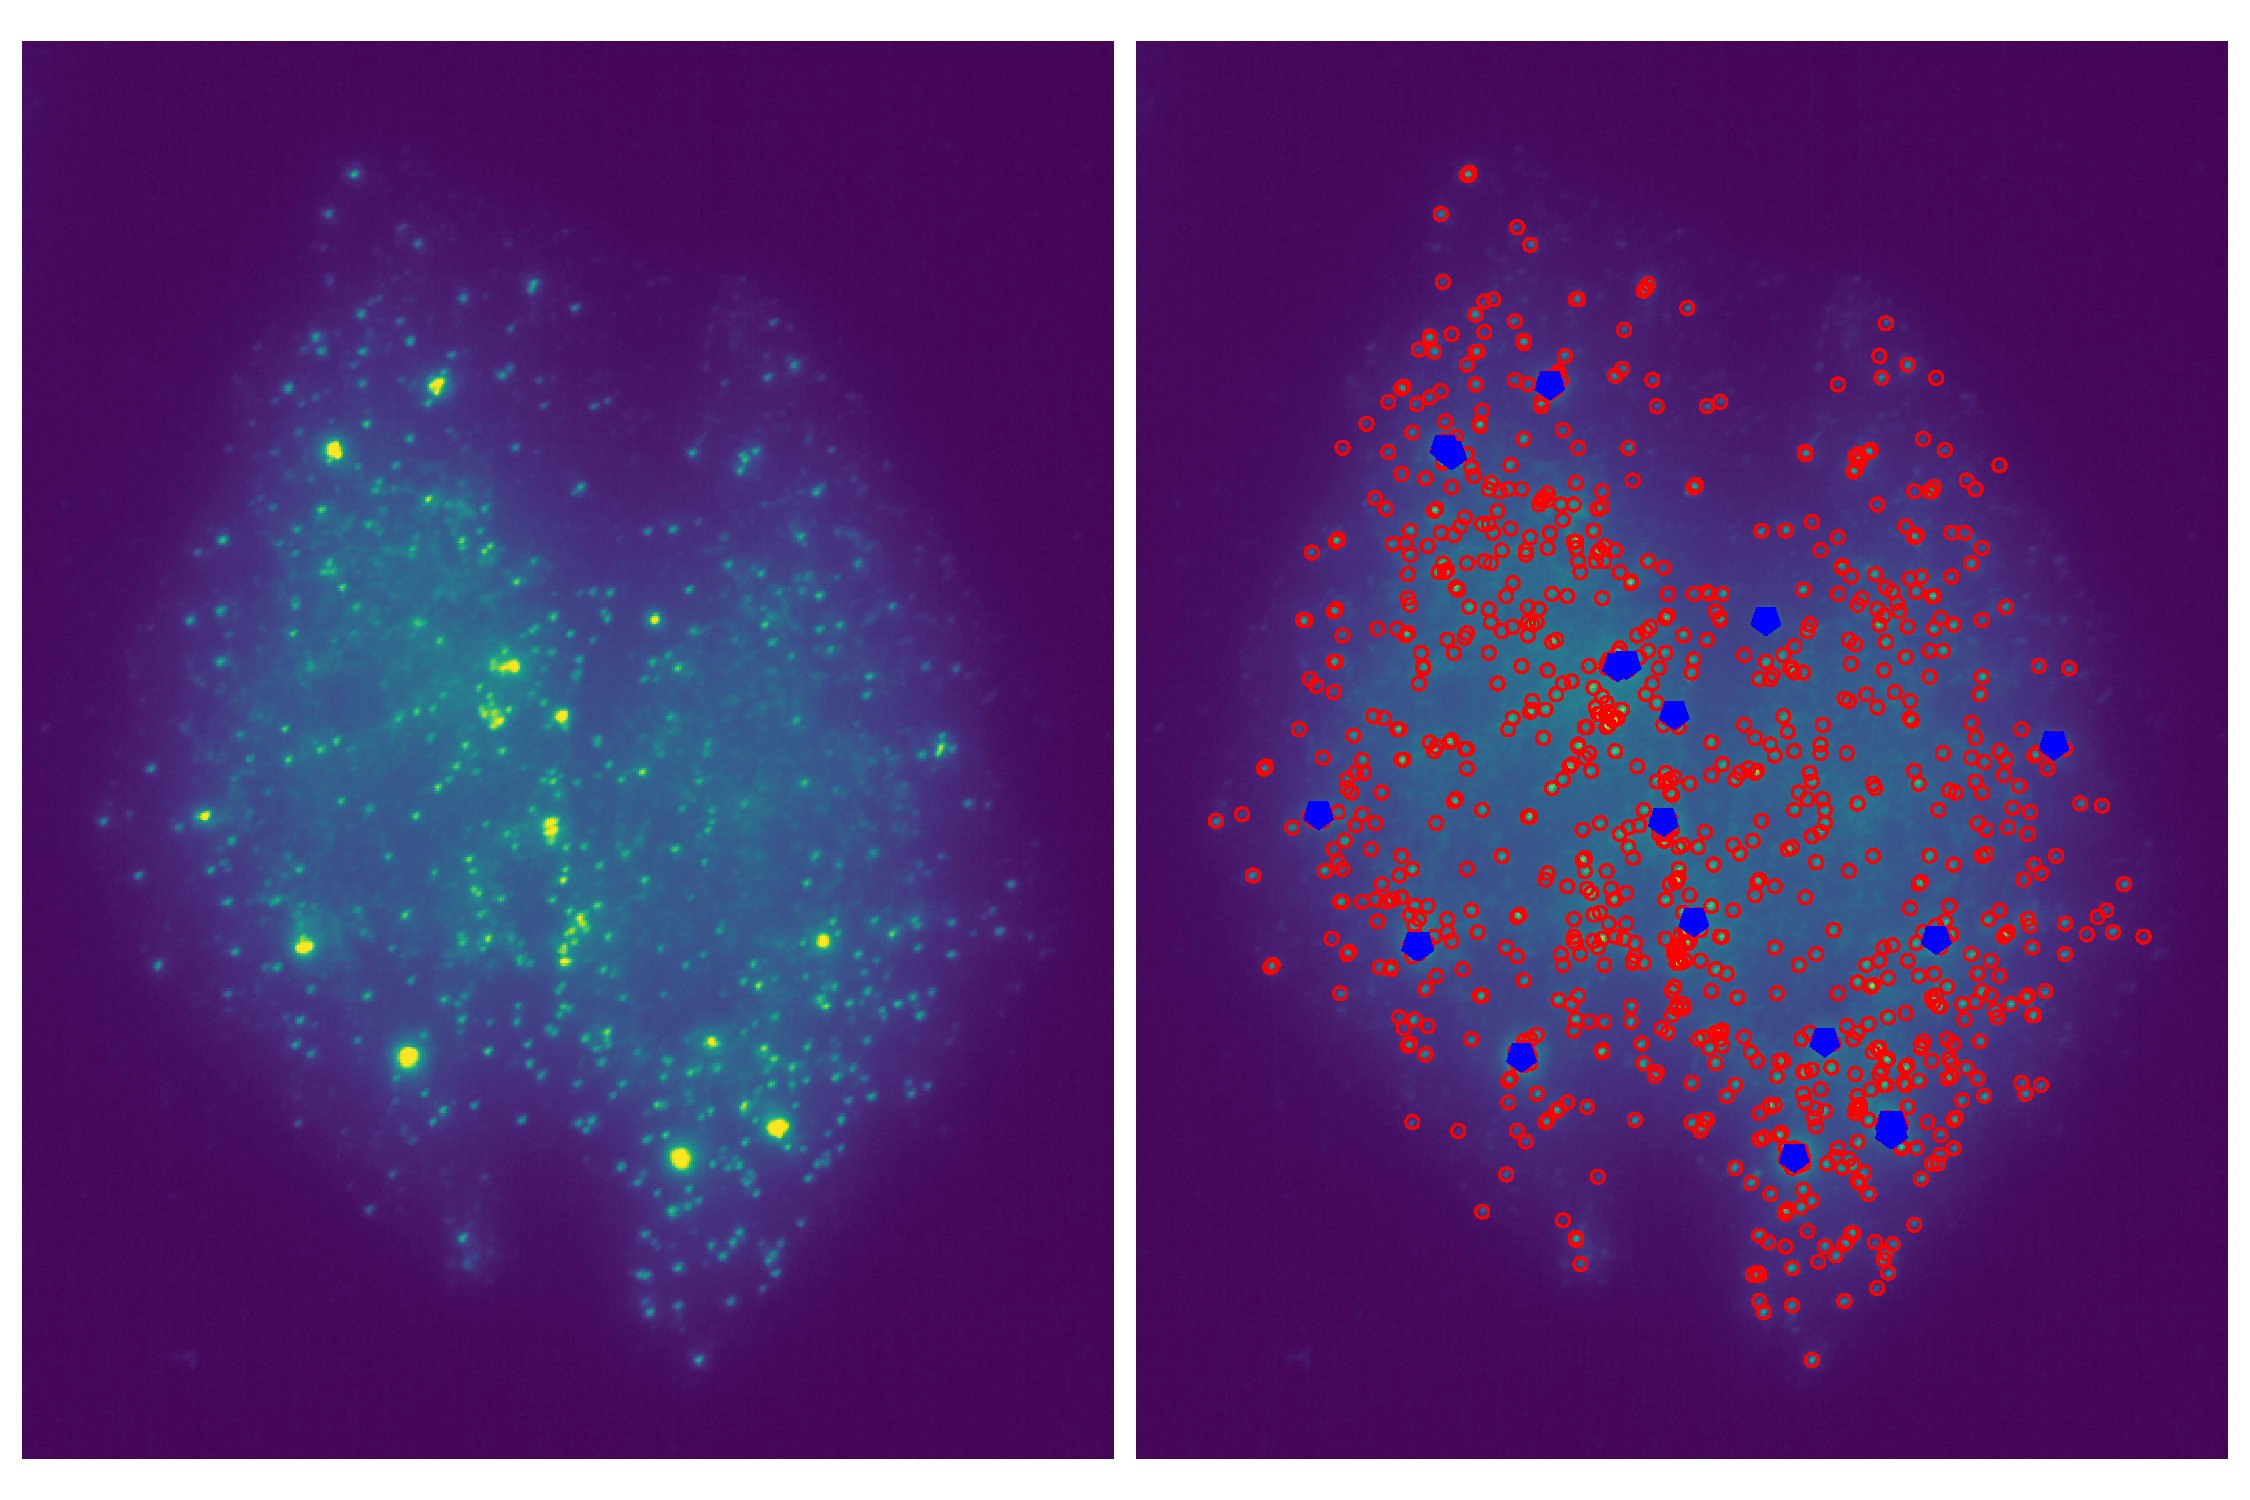
\includegraphics[width=1\textwidth]{figures/chapter2/cluster_detection_results}
    \caption{Blablabla}
    \label{fig:detection_results}
\end{figure}


The methods used to detect spots and to decompose foci are mainly adapted from
Aubin’s thesis. As mRNAs are usually smaller than diffraction limit, their measured
signal is a Point Spread Function (Point-Spread-Function (PSF)) (figure 7). The
microscope is not able to resolve such small objects. In
practice, we model this PSF by a 3-dimensional Gaussian function.
Spot detection Our spot detection pipeline consists in three steps that we can
easily adapt in three dimensions (using 3-dimensional filters):
• We filter the image to denoise the background and enhance the signal peaks.
• We detect these local peaks.
• We only keep the peaks above a fixed threshold.
Based on Aubin’s benchmark studies, we apply a Laplacian of Gaussian (LoG)
filter: we smooth the image (Gaussian filter) then an approximation of its
second derivative is computed (Laplacian filter). Another preprocessing consists
in estimating the background of the image (the lowest frequencies of the signal),
with a large Gaussian filter, then subtracting it from the original image. If a
second, and smaller, Gaussian filter is applied to smooth the resulting image,
we get a Difference of Gaussians (DoG) filter which is a faster approximation of
the LoG filter (figure 8). Both methods aim to remove the background signal and
increase the signal-to-noise ratio of the spots. The peak detection corresponds
to the detection of local maxima of the filtered image. We only keep local maxima
for which the filtered image has values exceeding a chosen threshold. In order
to detect isolated spots, we also apply an additional criterion on proximity,
i.e. we require that the selected spots are maximal in a certain neighborhood.

\section{Related work}

Hey, that's me: \cite{imbert_fish-quant_2022}.

\subsection{Classical methods}

I have visited \ac{IGMM}.

The second step, fluorescence spot detection, has been addressed by a number
of approaches in the lit- erature, and more recently solutions specifically
adapted to smFISH have been proposed. RS-FISH allows robust and accurate detection
of fluorescent spots in 2D and 3D through radial symmetry but requires parameter
tuning before being scaled to a large set of images (Bahry et al. 2021). DeepLink
is a parameter-free deep-learning-based method, but is currently only available
for 2D data and might require retraining (Eichenberger et al. 2021). Lastly,
assigning spot counts to segmentation results and the subsequent analysis of
RNA levels and/or RNA locali- zation requires custom-written code (Stoeger et al. 2015; Samacoits et al. 2018).

\subsection{RS-FISH}

\subsection{DeepSpot}


\section{Automated spot detection}


\subsection{Spot detection}

\begin{figure}[h]
    \centering
    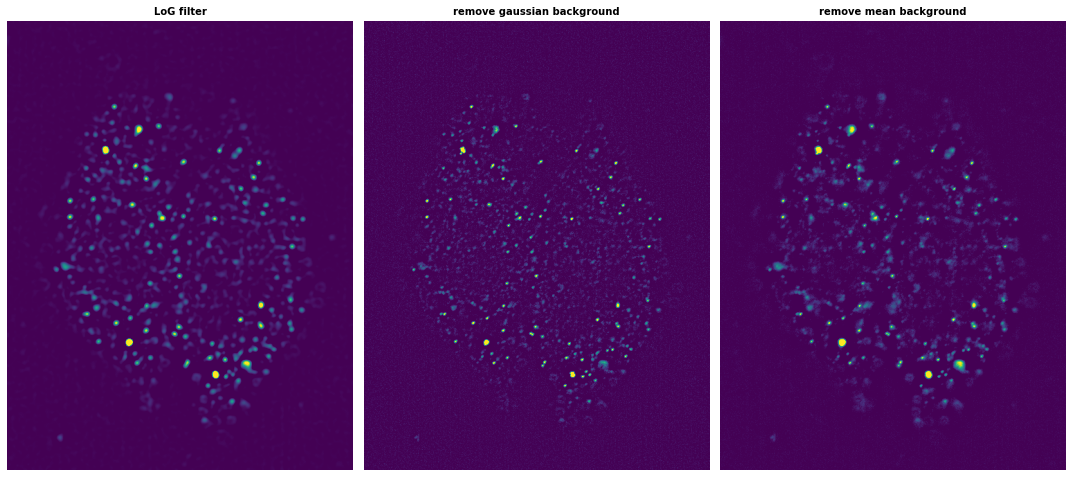
\includegraphics[width=1\textwidth]{figures/chapter2/filter_background}
    \caption{Blablabla}
    \label{fig:filter_remove_background}
\end{figure}

\subsection{Automated threshold}


\begin{wrapfigure}{L}{0.5\textwidth}
  \begin{center}
    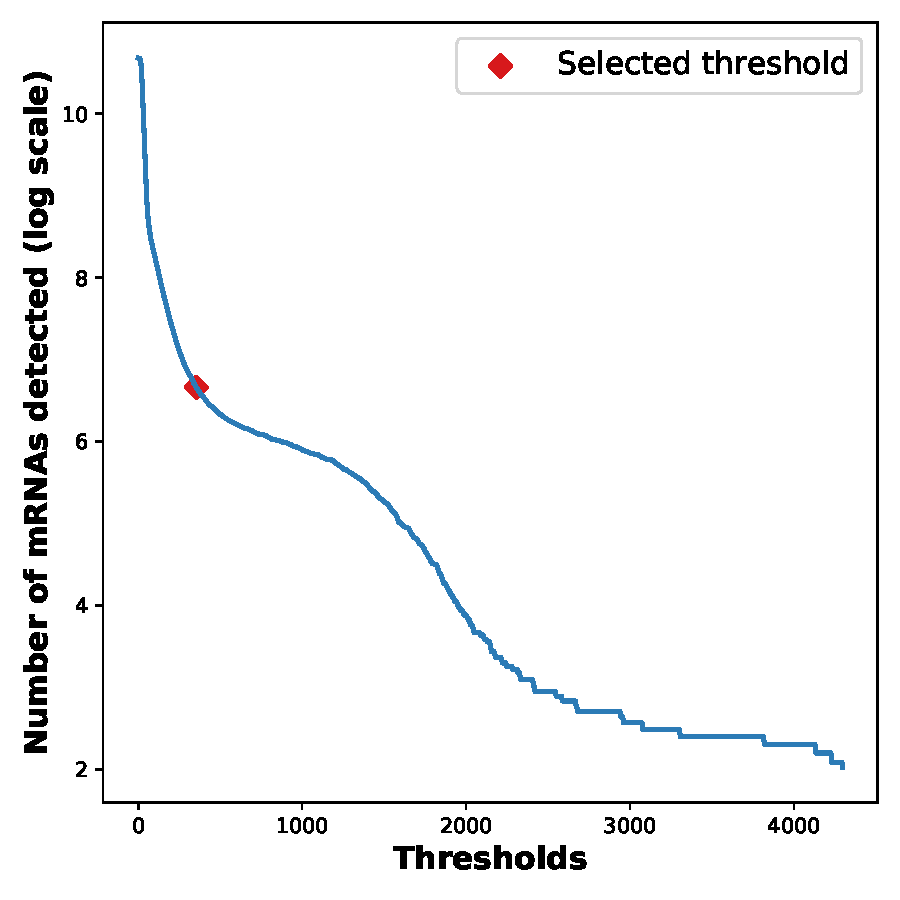
\includegraphics[width=0.33\textwidth]{figures/chapter2/elbow_curve_real}
  \end{center}
  \caption{Blablabla}
  \label{fig:elbow_detection}
\end{wrapfigure}


\begin{figure}[h]
    \centering
    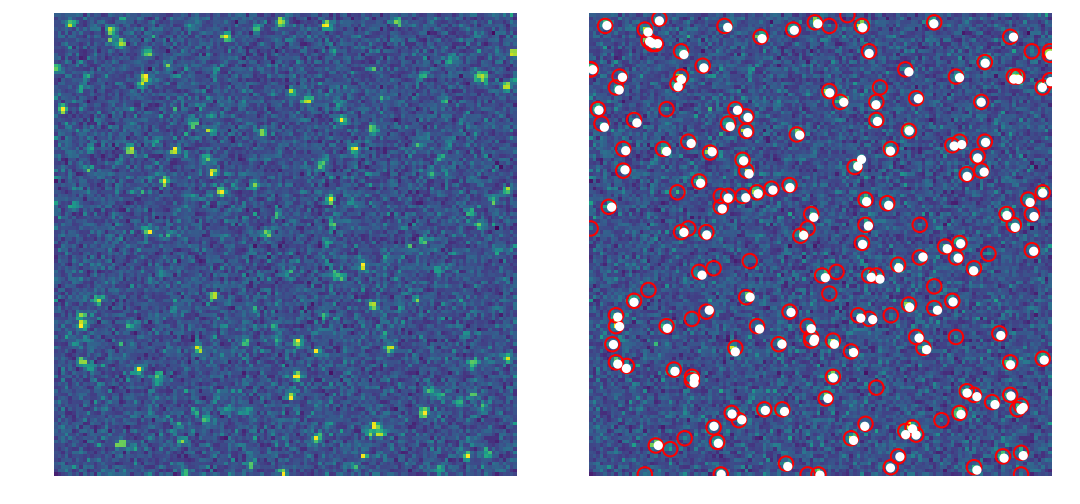
\includegraphics[width=1\textwidth]{figures/chapter2/plot_spot_detection}
    \caption{Blablabla}
    \label{fig:testAA}
\end{figure}


% code

\begin{minipage}{\linewidth}
\begin{lstlisting}[language=Python]
import bigfish.detection as detection

# spot detection with automated thresholding
spots, threshold = detection.detect_spots(
    images=rna,
    return_threshold=True,
    voxel_size=(300, 103, 103),  # in nanometer
    spot_radius=(350, 150, 150))  # in nanometer
\end{lstlisting}
\end{minipage}

\section{Dense region decomposition and cluster detection}

Foci decomposition Sometimes, mRNAs cluster together to build foci. In this
case, we are often not able to resolve the actual diffraction limited spots.
In order to quantitatively describe spatial mRNAs distributions, we therefore
need to decompose these foci into the constituting single spots. Of note, if
the foci are present in the cytoplasm, they represent a specific localization
pattern for the mRNAs, but inside the nuclei, they are most likely transcription
sites, which are irrelevant for our current projects.
We first select potential regions in the image which could host foci. Potential
foci are expected to be regions larger and brighter than spots. Such a region must
answer one or several of the following criteria:

• The region must be larger than isolated spots, i.e. we apply a size threshold.

• The region must be particularly bright, probably corresponding to several spots
on top of each other, i.e. we apply a threshold on the maximal pixel intensity in
the region.

• The region must contain several local maxima, corresponding to several detected
spots.

As in Aubin’s thesis, we first threshold the LoG filtered image with the same
threshold used to detect spots. While the spot detection used this threshold for
filtering local maxima, it is now applied as a pixel-wise threshold. For
decomposition, we only keep connected components meeting our criteria in term
of size, intensity and number of local maxima.
As we model a spot as a Gaussian signal, we fit a mixture of Gaussians in these
regions to estimate the number of mRNA molecules clustered. Fortunately, we
know that for a given gene, individual mRNAs have a reasonably similar PSF: while
the number of hybridizing probes can vary between individual molecules, we can
assume that these variations — for a given sequence — can be neglected. Hence,
we can estimate a realistic model for a typical spot by detecting isolated spots
(see above) and calculating their pixel-wise average or median (figure 7). We use
this reference spot to fit a Gaussian signal (amplitude and standard deviation).
These parameters are then used to simulate generic Gaussian signals corresponding
to realistic spots.

For each region, from an empty matrix, we add a simulated Gaussian signal centered
to the pixel with the maximum intensity of the region. We compute the difference
between the original image and our simulated Gaussian Mixture, then we repeat the
previous operation on this residual image. The iterative process stops when the
sum of squared residuals stops decreasing. The resulting simulated image reproduces
the original one with generic Gaussian signals and a background noise. The number
of Gaussians we add during this process is the estimated number of mRNAs in the
foci. After removing the spots initially detected in these regions, we get two
sets of spots coordinates: those inside a foci and those outside (figure 9).
Therefore, it is easy to filter the spots from a transcription site.

\subsection{Dense region detection}

\subsection{Dense region decomposition}

For each region, from an empty matrix, we add a simulated Gaussian signal centered
to the pixel with the maximum intensity of the region. We compute the difference
between the original image and our simulated Gaussian Mixture, then we repeat the
previous operation on this residual image. The iterative process stops when the
sum of squared residuals stops decreasing. The resulting simulated image reproduces
the original one with generic Gaussian signals and a background noise. The number
of Gaussians we add during this process is the estimated number of mRNAs in the
foci. After removing the spots initially detected in these regions, we get two
sets of spots coordinates: those inside a foci and those outside (figure 9).
Therefore, it is easy to filter the spots from a transcription site.


\begin{wrapfigure}{R}{0.33\textwidth}
  \begin{center}
    
\includegraphics[width=0.33\textwidth]{figures/chapter2/reference_spot}
  \end{center}
  \caption{Blablabla}
  \label{fig:reference_spot}
\end{wrapfigure}


\begin{figure}[h]
    \centering
    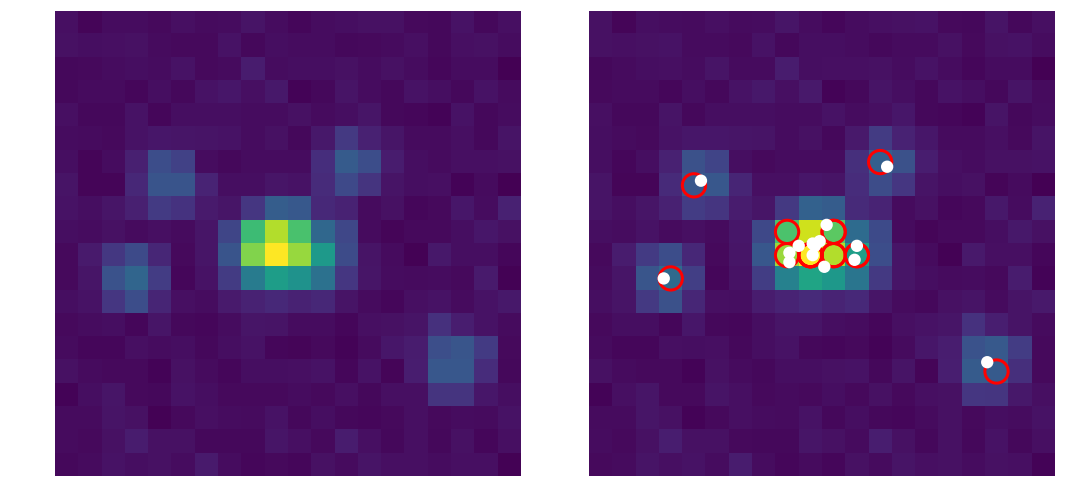
\includegraphics[width=1\textwidth]{figures/chapter2/plot_dense_decomposition}
    \caption{Blablabla}
    \label{fig:testD}
\end{figure}

% code

\subsection{Cluster detection}


\begin{figure}[h]
    \centering
    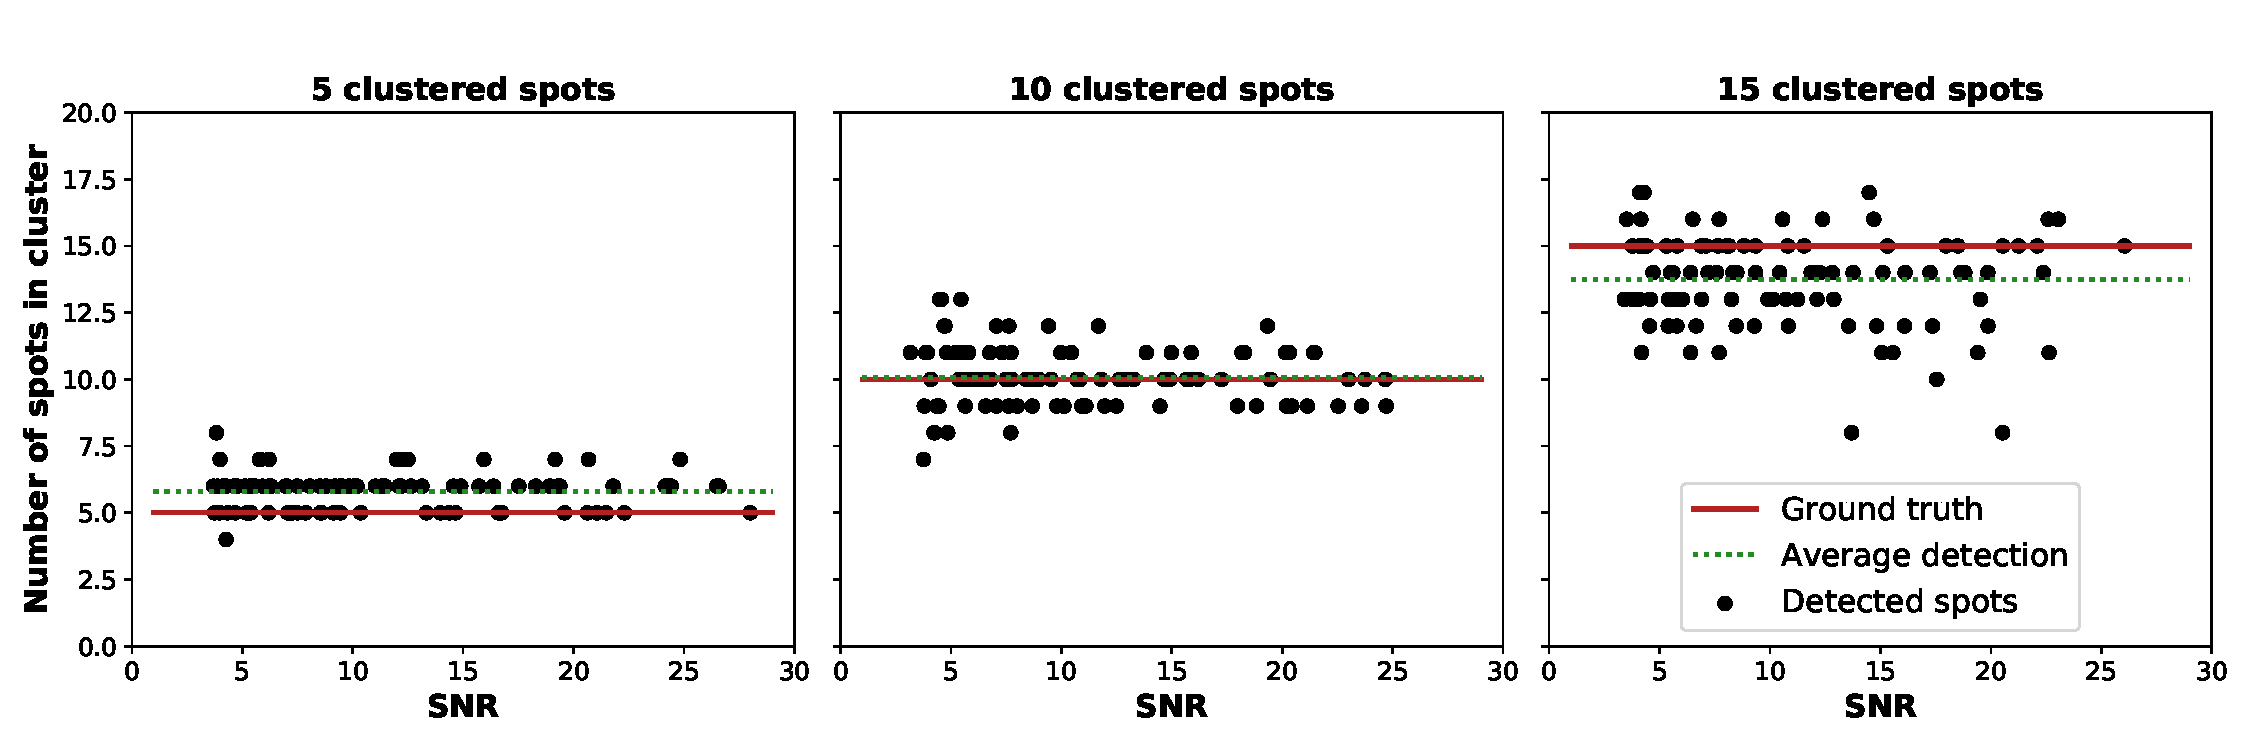
\includegraphics[width=1\textwidth]{figures/chapter2/cluster_along_noise}
    \caption{Blablabla}
    \label{fig:cluster_results}
\end{figure}

% code

\section{Additional features}

The detection subpackage implements the methods re- quired to detect spots in
2D or 3D images (Figs. 2, 3A–E). An important aspect of the detection subpackage
is its abil- ity to detect spots without setting any pixel intensity thresh- old.
We implemented a method to automatically infer this threshold from the image.
The curve describing the num- ber of detected spots as a function of the
intensity threshold (Fig. 3A,B) has an elbow shape, resulting from the superposition
of the fast decreasing false positive de- tections (low intensity noise) and the
slowly decreasing true positives. The threshold selected corresponds to the kink
in the elbow, and corresponds thus to the highest threshold outside the high-noise
regime. In order to val- idate this approach, we simulated real- istic smFISH images
with varying noise levels (Fig. 3A,B; Supplemental Note 1). We found that our method
only leads to a moderate over-estimation of detected spots (<5%–10%) for images with
moderate to high SNR values (>5). Such automatization over- comes human intervention
and allows scaling to large data sets, such that the subpackage can process thousands
of images. While initially designed to detect individual mRNAs, the same methods
can also be used to detect other spot-like structures (Safieddine et al. 2021),
such as centrosomes, P- bodies, etc (Fig. 3E).This subpackage further permits us
to perform localiza- tion of RNAs with subpixel accuracy by using a Gaussian
fitting (Mueller et al. 2013). Lastly, we provide the pos- sibility to perform
a colocalization analysis between spot detection per- formed in multiple channels (Cornes et al. 2021).


Strong local accumulation of RNAs, for example, active transcription sites, RNA
foci, or areas of local translation (Chouaib et al. 2020), can lead to an
underdetection since such accumula- tions are counted as single RNAs. For
such cases, we provide tools to decompose these dense regions and estimate
the number of spots based on our earlier work (Fig. 3C; Samacoits et al. 2018).
We validated this ap- proach again on simulated data (Fig 3D; see Supplemental Note 1),
and found consistent per- formance across relevant noise levels.

\subsection{Subpixel fitting}



\begin{figure}[h]
    \centering
    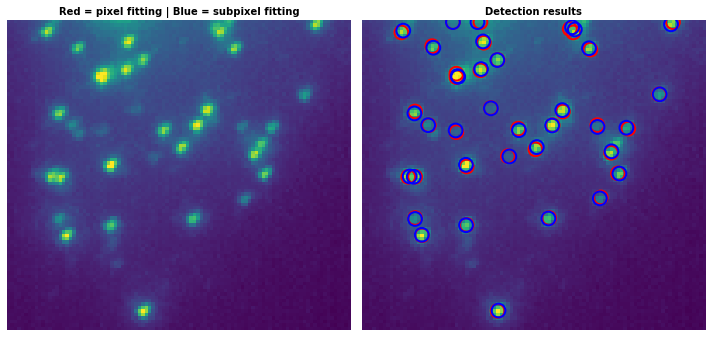
\includegraphics[width=1\textwidth]{figures/chapter2/subpixel_fitting}
    \caption{Blablabla}
    \label{fig:subpixel_fitting}
\end{figure}


% code

\subsection{Spot colocalization}


\begin{wrapfigure}{R}{0.5\textwidth}
  \begin{center}
    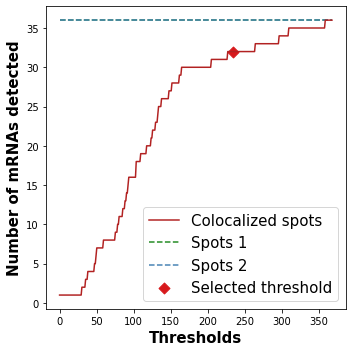
\includegraphics[width=0.33\textwidth]{figures/chapter2/colocalization_elbow}
  \end{center}
  \caption{Blablabla}
  \label{fig:elbow_colocalization}
\end{wrapfigure}

% code

% https://github.com/PreibischLab/RS-FISH/tree/master/documents/tool_comparison_for_paper